\newcommand{\svcourse}{CST Part IA: Introduction to Probability}
\newcommand{\svnumber}{1}
\newcommand{\svvenue}{Churchill, Room TBD}
\newcommand{\svdate}{2022-05-14}
\newcommand{\svtime}{11:00}
\newcommand{\svuploadkey}{PO5ogKIM8KQA22FZS8IAf8gxA8XKi19jxIBVHIfFZ+3GCBXuNUXS9lVN6bNYjxM/}

\newcommand{\svrname}{Mr Matthew Ireland}
\newcommand{\jkfside}{twoside}
\newcommand{\jkfhanded}{right}

\newcommand{\studentname}{Harry Langford}
\newcommand{\studentemail}{hjel2@cam.ac.uk}


\documentclass[10pt,\jkfside,a4paper]{article}

\usepackage{tikz}
\usepackage{mathtools}
\usepackage{tipa}
\usetikzlibrary{positioning, calc}

% DO NOT add \usepackage commands here.  Place any custom commands
% into your SV work files.  Anything in the template directory is
% likely to be overwritten!

\usepackage{fancyhdr}

\usepackage{lastpage}       % ``n of m'' page numbering
\usepackage{lscape}         % Makes landscape easier

\usepackage{verbatim}       % Verbatim blocks
\usepackage{epsfig}         % Embed encapsulated postscript
\usepackage{array}          % Array environment
\usepackage[nolinks]{qrcode}         % QR codes
\usepackage{enumitem}       % Required by Tom Johnson's exam question header

\usepackage{hhline}         % Horizontal lines in tables
\usepackage{siunitx}        % Correct spacing of units
\usepackage{amsmath}        % American Mathematical Society
\usepackage{amssymb}        % Maths symbols
\usepackage{amsthm}         % Theorems

\usepackage{ifthen}         % Conditional processing in tex

\usepackage[top=3cm,
            bottom=3cm,
            inner=2cm,
            outer=5cm]{geometry}

% PDF metadata + URL formatting
\usepackage[
            pdfauthor={\studentname},
            pdftitle={\svcourse, SV \svnumber},
            pdfsubject={},
            pdfkeywords={9d2547b00aba40b58fa0378774f72ee6},
            pdfproducer={},
            pdfcreator={},
            hidelinks]{hyperref}

\renewcommand{\headrulewidth}{0.4pt}
\renewcommand{\footrulewidth}{0.4pt}
\fancyheadoffset[LO,LE,RO,RE]{0pt}
\fancyfootoffset[LO,LE,RO,RE]{0pt}
\pagestyle{fancy}
\fancyhead{}
\fancyhead[LO,RE]{{\bfseries \studentname}\\\studentemail}
\fancyhead[RO,LE]{{\bfseries \svcourse, SV~\svnumber}\\\svdate\ \svtime, \svvenue}
\fancyfoot{}
\fancyfoot[LO,RE]{For: \svrname}
\fancyfoot[RO,LE]{\today\hspace{1cm}\thepage\ / \pageref{LastPage}}
\fancyfoot[C]{\qrcode[height=0.8cm]{\svuploadkey}}
\setlength{\headheight}{22.55pt}

\ifthenelse{\equal{\jkfside}{oneside}}{

 \ifthenelse{\equal{\jkfhanded}{left}}{
  % 1. Left-handed marker, one-sided printing or e-marking, use oneside and...
  \evensidemargin=\oddsidemargin
  \oddsidemargin=73pt
  \setlength{\marginparwidth}{111pt}
  \setlength{\marginparsep}{-\marginparsep}
  \addtolength{\marginparsep}{-\textwidth}
  \addtolength{\marginparsep}{-\marginparwidth}
 }{
  % 2. Right-handed marker, one-sided printing or e-marking, use oneside.
  \setlength{\marginparwidth}{111pt}
 }

}{
 % 3. Alternating margins, two-sided printing, use twoside.
}

\setlength{\parindent}{0em}
\addtolength{\parskip}{1ex}

% Exam question headings, labels and sensible layout (courtesy of Tom Johnson)
\setlist{parsep=\parskip, listparindent=\parindent}
\newcommand{\examhead}[3]{\section{#1 Paper #2 Question #3}}
\newenvironment{examquestion}[3]{
    \examhead{#1}{#2}{#3}\setlist[enumerate, 1]{label=(\alph*)}\setlist[enumerate, 2]{label=(\roman*)}
    \marginpar{\qrcode{https://www.cl.cam.ac.uk/teaching/exams/pastpapers/y#1p#2q#3.pdf}}
    \marginpar{\footnotesize \url{https://www.cl.cam.ac.uk/teaching/exams/pastpapers/y#1p#2q#3.pdf}}
}{}



\begin{document}

\begin{examquestion}{2004}{3}{7}

\begin{enumerate}

\item What is Turing's Thesis?

The Turing's Thesis states that any computable algorithm can be realised as
a Turing Machine.

This means that ``there is no model of computation which is \textit{more}
powerful than a Turing Machine''.

\item Explain the action of a Turing Machine that is specified by a
quintuplet description.

A Turing Machine is specified by a quadruple $M = (Q, \Sigma, s, \delta)$.

\begin{itemize}

\item $Q$ is the set of states

\item $\Sigma$ is the symbols in the language the machine $M$ reads

\item $s$ is the start state for the machine $M$

\item $\delta = (Q \times \Sigma) \to (Q \cup \{acc, rej\} \times \Sigma
 \times \{L, R, S\})$ is the transition function.

\end{itemize}

A Turing Machine performs (potentially infinite) computation and halts when
the state is either $acc$ or $rej$.

\item Define the \textit{configuration} of a Turing Machine at step $t$, and
establish equations that specify the configuration of a $k$-symbol Turing
machine at step $(t + 1)$ in terms of the configuration of the previous step
$t$.

A Turing Machine Configuration is a triple $(q, w, u)$ where $q \in Q$ is
the state of the Turing Machine, $w = va \in \Sigma \times \Sigma^*$ is the
list of symbols to the left of the tape head (including the symbol under the
tape head) and $u$ is the list of symbols to the right of the tape head.

At each step, the Turing Machine inspects $a$ (the last symbol in $w$) and
performs the action specified by $\delta(q, a)$. If $\delta(q, a) = (q',
\sigma, \{D\})$ then the Machine transitions into state $q'$, sets the
symbol underneath the head of the tape to $\sigma$ and moves in direction $D$.

The initial configuration of a Turing Machine is $(s, \triangleright, t)$
where $s$ is the start state, $\triangleright$ is the left endmarker.

With $c_t = (q, va, bu)$, and $\delta(q, a) = (q', \sigma, \{D\})$ the
configuration at time $t+1$, $c_{t+1}$ is given by:
\[
c_{t+1} =
\begin{cases}
(q', v, \sigma b u) & \ \text{if} \ D=L \\
(q', v\sigma, b u) & \ \text{if} \ D=S \\
(q', v\sigma b, u) & \ \text{if} \ D=R
\end{cases}
\]

\end{enumerate}

\end{examquestion}

\begin{examquestion}{2005}{3}{7}

\begin{enumerate}

\item Explain informally, i.e without reference to any particular model of
computation, why the \textit{Halting Problem} is undecidable.

By assuming the existence of a program that solves the Halting problem, we
can derive a contradiction.

\newcommand{\op}{\ensuremath{\textopencorner}}
\newcommand{\cl}{\ensuremath{\textcorner}}

Algorithms can be represented as integers. Assume there is some program
$P$ which solves the halting problem. When $P(e, a)$ is passed the integer
representation of a program $e$ and its arguments $a$, returns 1 if the
program halts when ran with those arguments and 0 if it does not halt.

Consider the algorithm $A'$ which when run with argument $e$, runs
$A(\op A' \cl, \op e \cl)$ loops infinitely if and only if it returns 1.
\begin{align*}
& A'(\op e \cl) \ \text{halts} \Longrightarrow \\
& A(\op A' \cl, \op e \cl) \ \text{returns 0} \Longrightarrow \\
& A'(\op e \cl) \ \text{does not halt}
\end{align*}
So the program $A'$ ran with any argument $\op e \cl$ halts if and only if
the program $A'$ ran with arguments $\op e \cl$ does not halt. This is a
contradiction. Since, $A'$ was constructed (computably) from the algorithm
$A$ we can conclude that no algorithm $A$ can exist. Therefore, there
exists no algorithm that solves the Halting Problem.

\item Briefly describe two mathematical problems, other than the
\textit{Halting Problem} that are algorithmically undecidable.

Two mathematical problems which are algorithmically
undecidable are the Entscheidungsproblem and whether or not there exist
solutions to Diophantine Equations.

\begin{itemize}

\item The Entscheidungsproblem asks for a proof there is an algorithm which
can determine in a finite number of steps whether or not there exists a proof
for any mathematical formula. This is an undecidable problem -- no such
algorithm exists.

\item Whether or not there is an integer solution to a Diophantine Equation
is undecidable.

A Diophantine equation is an equation consisting only of constants
multiplied by polynomial terms. For example $3 x^2 y^9 z - 93 x^4 y^3 = 0$.

\end{itemize}

\end{enumerate}

\end{examquestion}

\section{Exercise Sheet}

\begin{enumerate}

\setcounter{enumi}{3}

\item Show that there is a register machine computable partial function
$f: \mathbb{N} \rightharpoonup \mathbb{N}$ such that both
$\{x \in \mathbb{N}\ |\ f(x)\downarrow\}$ and
$\{y \in \mathbb{N}\ |\ (\exists x \in \mathbb{N}) f(x) = y\}$ are register
machine undecidable.

\[
f(e) =
\begin{cases}
e & \ \text{if}\ \phi_e(e)\downarrow

\end{cases}
\]

The definition of a register machine computable function is as follows:\\
A function $f: \mathbb{N}^n \rightharpoonup \mathbb{N}$ register machine
computable if and only if there exists a register machine with at least
$n + 1$ registers which when ran with $R_0=0$, $R_1=x_1, \dots, R_n=x_n$ and
all other registers zeroed will terminate with $R_0=y$ if and only if $f(x)=y$.

With $U$ as the Universal Register Machine, this register machine is given
below:
\begin{center}
\begin{tikzpicture}
\node (start) {\texttt{START}};
\node (r1minus) [below = of start] {$R_1^-$};
\node (r2plus) [below right = 0.6 of r1minus] {$R_2^+$};
\node (r3plus) [below left = 0.6 of r1minus] {$R_3^+$};
\node (r3minus) [right = of r1minus] {$R_3^-$};
\node (r1plus) [above = of r3minus] {$R_1^+$};
\node (halt) [right = of r3minus] {$U$};
\path [->] (start) edge (r1minus);
\path [->] (r1minus) edge (r3plus);
\path [->] (r3plus) edge (r2plus);
\path [->] (r2plus) edge (r1minus);
\path [->>] (r1minus) edge (r3minus);
\path [->] (r3minus) edge [bend left] (r1plus);
\path [->] (r1plus) edge [bend left] (r3minus);
\path [->>] (r3minus) edge (halt);
\node (r0zero) [right = of halt] {$R_0^-$};
\path [->] (r0zero) edge [loop above] (r0zero);
\node (r1minus2) [right = of r0zero] {$R_1^-$};
\node (r0plus) [below = of r1minus2] {$R_0^+$};
\path [->] (halt) edge (r0zero);
\node (halt) [above = of r1minus2] {\texttt{HALT}};
\path [->>] (r0zero) edge (r1minus2);
\path [->] (r1minus2) edge [bend left] (r0plus);
\path [->] (r0plus) edge [bend left] (r1minus2);
\path [->>] (r1minus2) edge (halt);
\end{tikzpicture}
\end{center}

If $\phi_e(e)$ does not halt, neither does this register machine. And if
$\phi_e(e)$ does halt, then this register machine halts with that value.
Therefore, this register machine computes the value of $f$.

If $\{x \in \mathbb{N}\ |\ f(x)\downarrow\}$ is decidable then we can solve
the halting problem. $\{y \in \mathbb{N}\ |\ (\exists x \in \mathbb{N}) f
(x) = y\}$ is similar -- if it were decidable then the halting
problem would be solved. However, since the halting problem is uncomputable,
a contradiction is reached and therefore both sets are uncomputable.

\item Suppose $S_1$ and $S_2$ are subsets of $\mathbb{N}$. Suppose
$f \in \mathbb{N} \to \mathbb{N}$ is a register machine computable function
satisfying: for all $x \in \mathbb{N}$, $x \in S_1 \Longleftrightarrow f(x)
\in S_2$. Show that $S_1$ is register machine decidable if $S_2$ is.

Assume $S_1$ is register machine decidable. Take an arbitrary $x$. Since $f$
is register-machine computable, we can compute $f(x)$. $S_2$ is decidable,
therefore we can determine whether $f(x)$ is in $S_2$. So we can determine
whether $x$ is in $S_1$. Since $x$ was arbitrary, we can conclude that if
$S_1$ is register machine decidable, then $S_1$ is register machine decidable.

\item Show that the set of codes $ \langle e, e' \rangle $ of pairs of
numbers $e$ and $e'$ satisfying $\phi_e = \phi_{e'}$ is undecidable.

Let $e$ be the integer representation of the register machine which is
constantly 0. Let $e'$ be arbitrary. In order to determine whether
$\phi_{e'} = \phi_e$, we must now determine whether $\phi_{e'}$ halts with
value 0 on all inputs. Consider an arbitrary input $x$. We must now
determine whether $\phi_{e'}(x)$ halts with value 0. So we must establish
whether $\phi_{e'}(x)$ halts -- this is uncomputable. Therefore, it's
uncomputable to determine whether $\phi_{e'} = \phi_e$ and therefore the set
of codes $ \langle e, e' \rangle $ of pairs such that $\phi_e = \phi_{e'}$
is undecidable.

\end{enumerate}

\section{Decidable Sets}

\begin{enumerate}[label=(\alph*)]

\item Show that decidable sets are closed under union, intersection and
complementation.

A set $S$ is decidable if and only if its characteristic function $\chi_S(x) =
\begin{cases} 0 & \ \text{if} \ x \in S \\ 1 & \ \text{otherwise} \
\end{cases}$ \\ is computable. Let $M_S$ be a register machine which computes
the characteristic function for the set $S$.

Define the new register machine $M_S'$ as follows:
\begin{center}
\begin{tikzpicture}
\node (start) {\texttt{START}};
\node (m) [right = of start] {$M_S$};
\node (r0minus) [right = of m] {$R_0^-$};
\node (r0plus) [right = of r0minus] {$R_0^+$};
\node (halt) [right = of r0plus] {\texttt{HALT}};
\path [->]  (start) edge (m);
\path [->]  (m) edge (r0minus);
\path [->>] (r0minus) edge (r0plus);
\path [->]  (r0minus) edge [bend left] (halt);
\path [->]  (r0plus) edge (halt);
\end{tikzpicture}
\end{center}

The result of the register machine $M_S'$ is given by:
\[
M_S'(x) =
\begin{cases}
0 & \ \text{if} \ M_S(x) = 1 \\
1 & \ \text{otherwise}
\end{cases}
= \begin{cases}
0 & \ \text{if} \ x \in S \\
1 & \ \text{otherwise}
\end{cases}
= \begin{cases}
1 & \ \text{if} \ x \in \bar{S} \\
0 & \ \text{otherwise}
\end{cases}
\]
So the machine $M_S'$ computes the complement of the set $S$. Since $S$ was
an arbitrary decidable set we can conclude that decidability is closed
under complementation.

\item Do these closure properties hold for undecidable languages?

The closure property only holds for complementation.

Assume there exists some arbitrary undecidable set $S$ such that the
complement of $S$, $\bar{S}$ is decidable. If $\bar{S}$ is decidable, then
its characteristic function $\chi_{\bar{S}}$ is decidable. Decidability is
closed under function composition. Therefore $f \circ \chi_{\bar{S}}$ is
also computable for $f = \{(0, 1), (1, 0)\}$. So $f \circ \chi_{\bar{S}} =
\chi_S$. So the characteristic function for $S$ is computable and therefore
$S$ is decidable. However, this contradicts the original assumption that $S$
was undecidable. Therefore, there can exist no undecidable set $S$ such
that its complement $\bar{S}$ is computable. Hence undecidability is closed
under complementation.

I prove undecidability is not closed under intersection and union by
example. Consider the undecidable set $S$ and its complement $\bar{S}$.

$S \cap \bar{S} = \emptyset$ -- $\emptyset$ is decidable and therefore
undecidability is not closed under intersection.

$S \cap \bar{S} = \mathbb{N}$ -- $\mathbb{N}$ is decidable and therefore
undecidability is not closed under intersection.

\end{enumerate}

\begin{examquestion}{2006}{3}{7}

\begin{enumerate}

\item Give a graphical representation of the following register machine
program.
\begin{align*}
L0 &: Z^+ \to L1 \\
L1 &: L^- \to L2, L3 \\
L2 &: Z^+ \to L0 \\
L3 &: Z^- \to L4, L5 \\
L4 &: L^+ \to L3 \\
L5 &: X^- \to L1, L6 \\
L6 &: \texttt{HALT}
\end{align*}

\begin{center}
\begin{tikzpicture}
\node (start) {\texttt{START}};
\node (z-plus) [below = of start] {$Z^+$};
\node (l-minus) [right = of z-plus] {$L^-$};
\node (z-minus) [right = of l-minus] {$Z^-$};
\node (x-minus) [right = of z-minus] {$X^-$};
\node (tmp) [right = 0.5 of z-plus] {};
\node (z-plus2) [below = 0.866 of tmp] {$Z^+$};
\node (l-plus) [below = of z-minus] {$L^+$};
\node (halt) [above = of x-minus] {\texttt{HALT}};
\path [->] (start) edge (z-plus);
\path [->] (z-plus) edge (l-minus);
\path [->>] (l-minus) edge (z-minus);
\path [->>] (z-minus) edge (x-minus);
\path [->] (l-minus) edge (z-plus2);
\path [->] (z-plus2) edge (z-plus);
\path [->] (z-minus) edge [bend left] (l-plus);
\path [->] (l-plus) edge [bend left] (z-minus);
\path [->>] (x-minus) edge (halt);
\path [->] (x-minus) edge [bend right] (l-minus);
\end{tikzpicture}
\end{center}

\item Assuming the contents of register $Z$ is initially 0, when the program
is run starting at instruction $L0$ what functions of the initial contents
of registers $X$ and $L$ are computed in $X$ and $L$ when the machine halts.

This is \texttt{PUSH} from the lectures. It pushes the contents of $X$ onto
the list held in $L$. So given an initial state of $(X, L)$, the final state
is given by $2^{X}(2 \cdot L + 1)$.

\item

\begin{enumerate}

\item What is meant by a Turing Machine, it's \textit{configurations},
\textit{transition relation} and the \textit{computations} is carries out?
What does it mean to say that a computation \textit{halts}.

A Turing Machine is a theoretical model of computation which recognises the
language of recursively enumerable grammars -- a function is computable if
and only if it can be computed on a Turing Machine.

Turing Machines can be described as a quadruple: $(Q, \Sigma, s, \delta)$.
$Q$ is the set of states the Turing Machine can be in (N.B.\@ $acc, rej \in
Q$), $\Sigma$ is the set of symbols which can be on the Turing Machine tape,
$s \in Q$ is the initial state and $\delta \subseteq (\Sigma \times Q) \to
(Q \times \Sigma \times \{L, S, R\})$ is the transition function.

A Turing Machine configuration is given by a triple $(q, w, u)$, where $q$
is the state the Turing Machine is currently in, $w \in \{\triangleright\}
\times \Sigma^*$ is the list of symbols on the tape to the left of the head
(including the one under the head) and $u \in \Sigma^*$ is the list of
non-blank symbols to the right of the head.

A Turing Machine starts in the configuration $(s, \triangleright, u )$ and
follows the transition function. If the Turing Machine is in state
$(q, wa, u)$ and $\delta(a, u) = (q', a', d)$ then the Turing Machine
moves into state $q'$, overwrites the current symbol with $a'$ and moves in
direction $d$.

A computation halts if the Turing Machine state ever reaches $acc$ or $rej$.

\item Given a Turing Machine, is it decidable whether or not for all
possible initial configurations the machine will not halt after 100 steps of
transitions? Justify your answer.

It is decidable. A Turing Machine with less than 100 transitions looks at at
most 100 symbols on the tape.

Since the number of possibilities that symbol can be is finite, the set of
initial configurations distinguishable within 100 steps is also finite
$\left(|\Sigma|^{100}\right)$. So we can enumerate all distinguishable
initial configurations and check whether the Turing Machine halts for all of
them. This method applies for any \textit{finite} number of steps $n$.

\end{enumerate}

\end{enumerate}

\end{examquestion}

\section{Exercise Sheet}

\begin{enumerate}

\setcounter{enumi}{6}

\item For the example Turing machine given on slide 64, give the register
machine program implementing $(S, T, D) \coloneqq \delta(S, T)$ as described
on slide 70. [Tedious! -- maybe just do a bit.]

\begin{align*}
Q &= \text{current state }, \{s \mapsto 0, q \mapsto 1, q' \mapsto 2, acc
\mapsto 3, rej \mapsto 4\} \\
A &= \text{current tape symbol }, \{\triangleright \mapsto 0, \_ \mapsto 1, 0
\mapsto 2, 1 \mapsto 3\} \\
D &= \text{current direction of tape head }, \{L \mapsto 0, R \mapsto 1, S
\mapsto 2\} \\
L &= \text{symbols to the left of the head} \\
R &= \text{symbols to the right of the head}
\end{align*}

\begin{center}
\begin{tikzpicture}
\node (start) {\texttt{START}};
\node (pop-l-to-a) [right = of start] {$A=L.pop()$};
\node (q-minus1) [below = 0.8 of pop-l-to-a] {$Q^-$};
\node (a-minus1) [below = 0.8 of q-minus1] {$A^-$};
\node (d-equals2) [right = of a-minus1] {$D\coloneqq 1$};

\node (push-a-to-r) [right = of pop-l-to-a] {$R=A.pop()$};
\node (d-minus1) [right = of push-a-to-r] {$D^-$};
\node (d-minus2) [above = 0.8 of d-minus1] {$D^-$};
\node (d-minus3) [above = 0.8 of d-minus2] {$D^-$};
\node (l-push-a) [left = of d-minus3] {$L.push(A)$};
\node (r-pop-a) [left = of l-push-a] {$A=R.pop()$};
\path [->] (start) edge (pop-l-to-a);
\path [->] (pop-l-to-a) edge (q-minus1);
\path [->] (q-minus1) edge (a-minus1);
\path [->>] (a-minus1) edge (d-equals2);
\path [->] (d-equals2) edge [bend right] (d-minus1);
\path [->>] (d-minus1) edge (push-a-to-r);
\path [->] (push-a-to-r) edge (pop-l-to-a);
\path [->] (d-minus1) edge (d-minus2);
\path [->>] (d-minus2) edge [bend right, out=-15, in=200] (q-minus1);
\path [->] (d-minus2) edge (d-minus3);
\path [->>] (d-minus3) edge (l-push-a);
\path [->] (l-push-a) edge (r-pop-a);
\path [->] (r-pop-a) edge [bend right, out=-60, in=240] (q-minus1);

\node (a-minus2) [below = 0.8 of a-minus1] {$A^-$};
\node (a-set1) [right = of a-minus2] {$A\coloneqq 1$};
\node (q-set1) [right = of a-set1] {$Q \coloneqq 1$};
\node (dset2) [right = of q-set1] {$D \coloneqq 1$};
\path [->] (a-minus1) edge (a-minus2);
\path [->>] (a-minus2) edge (a-set1);
\path [->] (a-set1) edge (q-set1);
\path [->] (q-set1) edge (dset2);
\path [->] (dset2) edge [bend right] (d-minus1);

\node (a-minus3) [below = 0.8 of a-minus2] {$A^-$};
\node (a-set2) [right = of a-minus3] {$A\coloneqq 2$};
\node (q-set4) [right = of a-set2] {$Q\coloneqq 4$};
\node (dset2) [right = of q-set4] {$D\coloneqq 2$};
\path [->] (a-minus2) edge (a-minus3);
\path [->>] (a-minus3) edge (a-set2);
\path [->] (a-set2) edge (q-set4);
\path [->] (q-set4) edge (dset2);
\path [->] (dset2) edge [bend right, out=-45, in=-135] (d-minus1);

\node (a-minus4) [below = 0.8 of a-minus3] {$A^-$};
\node (a-set3) [right = of a-minus4] {$A\coloneqq 3$};
\node (q-set4) [right = of a-set3] {$Q\coloneqq 4$};
\node (dset2) [right = of q-set4] {$D\coloneqq 2$};
\path [->] (a-minus3) edge (a-minus4);
\path [->>] (a-minus4) edge (a-set3);
\path [->] (a-set3) edge (q-set4);
\path [->] (q-set4) edge (dset2);
\path [->] (dset2) edge [bend right, out=-60, in=-120] (d-minus1);

\node (invis) [below = 0.5 of a-minus4] {$\vdots$};
\path [->] (q-minus1) edge [bend right] (invis);
\end{tikzpicture}
\end{center}

I've shown only part of the diagram. The other cases continue where
$\vdots$ is. There will be two more cases similar to the one shown for $q$
and $q'$. The cases for \texttt{acc} and \texttt{rej} will halt. For
brevity, I've omitted \texttt{halts} in $D^-$ and $A^-$ where they're not
possible due to invariants maintained by the Turing Machine. I further
assume that $X=L.pop()$ will set $X$ to $0$ if $L=0$ (the list
corresponding to the integer $L$ is empty).

\item Show that the following recursive functions are all primitive recursive

\begin{enumerate}

\item Exponentiation, $\exp \in \mathbb{N}^2 \to \mathbb{N}$.

\newcommand{\proj}[2]{\ensuremath{\text{proj}^{#1}_{#2}}}
\newcommand{\suc}{\text{succ}}
\newcommand{\zero}[1]{\ensuremath{\text{zero}^{#1}}}
\newcommand{\add}{\text{add}}
\newcommand{\mul}{\text{mul}}

\begin{align*}
&\begin{cases}
\add(x, 0) &\equiv \suc \circ x \\
\add(x, y+1) &\equiv \suc \circ \add(x, y)
\end{cases}\\
&\begin{cases}
\mul(x, 0) &= \zero{1}(x) \\
\mul(x_1, x + 1) &= \add(x_1, \mul(x_1, x))
\end{cases}\\
&\begin{cases}
\exp(x_1, 0) &\equiv \suc \circ \zero{1} \\
\exp(x_1, x + 1) &\equiv \mul(x_1, \exp(x_1, x))
\end{cases}
\end{align*}

\newcommand{\pred}{\text{pred}}
\newcommand{\minus}{\text{minus}}
\item Truncated subtraction, $ minus \in \mathbb{N}^2 \to \mathbb{N} $.
\begin{align*}
&\begin{cases}
\pred(0) &\equiv \zero{0} \\
\pred(x+1) &\equiv \proj{2}{1}(x, \pred(x))
\end{cases}\\
&\begin{cases}
\minus(x_1, 0) &\equiv \zero{1} \\
\minus(x_1, x+1) &\equiv \pred \circ \minus(x, y)
\end{cases}
\end{align*}

\newcommand{\iz}{\text{ifzero}}

\item Conditional branch on zero, $\iz \in \mathbb{N}^3 \to \mathbb{N}$.
\[
\begin{cases}
\iz(0, y, z)		&\equiv \proj{2}{1}(y, z) \\
\iz(x + 1, y, z)	&\equiv \proj{3}{3}(\iz(x, y, z), y, z)
\end{cases}
\]

\newcommand{\rx}{\ensuremath{\overrightarrow{x}}}
\item Bounded summation: if $f \in \mathbb{N}^{n+1} \to \mathbb{N}$ is
primitive recursive then so is $g \in \mathbb{N}^{n+1} \to \mathbb{N}$ where
\begin{align*}
&\begin{cases}
g(\rx, 0) &\equiv \zero{n}(\rx) \\
g(\rx, x + 1) &\equiv \add(f(\rx, x), g(\rx, x))
\end{cases}
\end{align*}

\end{enumerate}

\item Recall the definition of Ackermann's function $ack$. Sketch how to
build a register machine $M$ that computes $ack(x_1, x_2)$ in $R_0$ when
started with $x_1$ in $R_1$ and $x_2$ in $R_2$ ad all other registers zero.

Using registers as follows:
\begin{align*}
R_1 &= x_1 \ \text{in current call to Ack} \\
R_2 &= x_2 \ \text{in current call to Ack} \\
L &= \text{stack of $x_2$s} \\
Z_1 &= \text{temporary} \\
Z_2 &= \text{temporary}
\end{align*}
Whenever the top-left $R_1^-$ is run, the machine is at the start of a
function call. If it has to recurse, it pushes the value of $x_1$ for the
outermost call onto $L$ and performs the innermost call. In the base case
$Ack(0, x_2) = x_2+1$, if the stack is empty, return $x+1$ else pop the top of
the stack into $x_1$.
\begin{center}
\begin{tikzpicture}
\node (start) {\texttt{START}};
\node (r1minus) [below = of start] {$R_1^-$};
\node (r2minus1) [right = of r1minus] {$R_2^-$};
\node (r4plus1) [right = of r2minus1] {$Z_1^+$};
\node (r3minus) [right = of r4plus1] {$L^-$};
\node (r4minus) [right = of r3minus] {$Z_1^-$};
\node (r3plus) [below = of r4minus] {$L^+$};
\node (r4plus2) [left = 1.8 of r3plus] {$Z_1^+$};
\node (r1minus2) [right = of r4minus] {$R_1^-$};
\node (r5plus) [above = of r4minus] {$Z_2^+$};
\node (r1plus) [right = of r1minus2] {$R_1^+$};
\node (r5minus) [above = of r1plus] {$Z_2^-$};
\path [->] (start) edge (r1minus);
\path [->] (r1minus) edge (r2minus1);
\path [->] (r2minus1) edge (r4plus1);
\path [->] (r4plus1) edge (r3minus);
\path [->] (r3minus) edge (r4plus2);
\path [->] (r4plus2) edge (r4plus1);
\path [->>] (r3minus) edge (r4minus);
\path [->] (r4minus) edge [bend left] (r3plus);
\path [->] (r3plus) edge [bend left] (r4minus);
\path [->>] (r4minus) edge (r1minus2);
\path [->] (r1minus2) edge (r5plus);
\path [->] (r5plus) edge (r3minus);
\path [->>] (r1minus2) edge (r1plus);
\path [->] (r1plus) edge [bend left] (r5minus);
\path [->] (r5minus) edge [bend left] (r1plus);
\path [->>] (r5minus) edge [bend right] (r1minus);

\node (r2plus-case2) [below = of r2minus1] {$R_2^+$};
\path [->>] (r2minus1) edge (r2plus-case2);
\path [->] (r2plus-case2) edge (r1minus);

\node (r2plus-case3) [below = of r1minus] {$R_2^+$};
\node (r3minus-case3) [below = of r2plus-case3] {$L^-$};
\node (r2minus-case3) [below = of r3minus-case3] {$R_2^-$};
\node (r0plus-case3) [right = of r2minus-case3] {$R_0^+$};
\node (halt) [below = of r2minus-case3] {\texttt{HALT}};
\path [->>] (r1minus) edge (r2plus-case3);
\path [->] (r2plus-case3) edge (r3minus-case3);
\path [->>] (r3minus-case3) edge (r2minus-case3);
\path [->] (r2minus-case3) edge [bend left] (r0plus-case3);
\path [->] (r0plus-case3) edge [bend left] (r2minus-case3);
\path [->>] (r2minus-case3) edge (halt);

\node (r3plus-case3) [right = of r3minus-case3] {$L^+$};
\node (r3minus2-case3) [right = of r3plus-case3] {$L^-$};
\node (r4plus-case3) [below = of r3minus2-case3] {$Z_1^+$};
\node (r4minus1-case3) [right = of r3minus2-case3] {$Z_1^-$};
\node (r4minus2-case3) [right = of r4minus1-case3] {$Z_1^-$};
\node (r1plus-case3) [below = of r4minus1-case3] {$R_1^+$};
\node (r3plus2-case3) [below = of r4minus2-case3] {$L^+$};
\path [->] (r3minus-case3) edge (r3plus-case3);
\path [->] (r3plus-case3) edge (r3minus2-case3);
\path [->] (r3minus2-case3) edge [bend left] (r4plus-case3);
\path [->] (r4plus-case3) edge [bend left] (r3minus2-case3);
\path [->>] (r3minus2-case3) edge (r4minus1-case3);
\path [->>] (r4minus1-case3) edge (r1plus-case3);
\path [->] (r1plus-case3) edge (r3minus2-case3);
\path [->] (r4minus1-case3) edge (r4minus2-case3);
\path [->] (r4minus2-case3) edge (r3plus2-case3);
\path [->] (r3plus2-case3) edge (r4minus1-case3);
\path [->>] (r4minus2-case3) edge [bend left, out=10, in=130]
(r1minus);
\end{tikzpicture}
\end{center}

\end{enumerate}

\section{Minimisation}

Use minimisation to show that the following partial functions are 
partial recursive:

\begin{enumerate}

\item The binary maximum function $\max:\mathbb{N}^2 \to \mathbb{N}$
\[
\begin{cases}
\max(x, 0) &\equiv x \\
\max(x, y) &\equiv \text{ifzero}(\text{pred}(\text{minus}(x, y)), \text{succ}(y), x)
\end{cases}
\]

\item The integer square root function $\text{sqrt} \mathbb{N} \to
\mathbb{N}$, which is only defined if its argument is a perfect square.
\begin{align*}
&\begin{cases}
\text{equals}(x_1, 0) &\equiv \text{ifzero}(x_1, 0, 1) \\
\text{equals}(x_1, x + 1) &\equiv \text{ifzero}(\max(x_1, x), 0, 1)
\end{cases}\\
&\begin{cases}
\text{sqrt}(0) &\equiv 0 \\
\text{sqrt}(x + 1) &\equiv \mu^2\text{equals}(x + 1, \text{mul}(i, i))
\end{cases}
\end{align*}

\end{enumerate}

\end{document}